\documentclass[preprint]{aastex}
%\documentclass{emulateapj}


% has to be before amssymb it seems
%\usepackage{color,hyperref}
%\definecolor{linkcolor}{rgb}{0,0,0.5}
%\hypersetup{colorlinks=true,linkcolor=linkcolor,citecolor=linkcolor,
%            filecolor=linkcolor,urlcolor=linkcolor}
%\usepackage{amssymb,amsmath}

\usepackage{color}
\usepackage{url}
\usepackage{graphicx}
\graphicspath{{figures/}}

% For Python code
\usepackage{listings}
\definecolor{lbcolor}{rgb}{0.9,0.9,0.9}
\lstset{language=Python,
        basicstyle=\footnotesize\ttfamily,
        showspaces=false,
        showstringspaces=false,
        tabsize=2,
        breaklines=false,
        breakatwhitespace=true,
        identifierstyle=\ttfamily,
        keywordstyle=\bfseries\color[rgb]{0.133,0.545,0.133},
        commentstyle=\color[rgb]{0.133,0.545,0.133},
        stringstyle=\color[rgb]{0.627,0.126,0.941},
    }

% Draft watermark:
%\usepackage{draftwatermark}
%\SetWatermarkLightness{0.9}
%\SetWatermarkScale{4}

% Some macros
\newcommand{\todo}[1]{{\color{red} [TODO: #1]}}
\newcommand{\foreign}[1]{{\it #1}}

\newcommand{\apriori}{\foreign{a priori}}
\newcommand{\adhoc}{\foreign{ad hoc}}
\newcommand{\etal}{\foreign{et\,al.}}
\newcommand{\etc}{\foreign{etc.}}

\newcommand{\Fig}[1]{Figure~\ref{fig:#1}}
\newcommand{\fig}[1]{\Fig{#1}}
\newcommand{\figlabel}[1]{\label{fig:#1}}
\newcommand{\Eq}[1]{Equation~(\ref{eq:#1})}
\newcommand{\eq}[1]{\Eq{#1}}
\newcommand{\eqs}[2]{Equations~(\ref{eq:#1})-(\ref{eq:#2})}
\newcommand{\eqlabel}[1]{\label{eq:#1}}
\newcommand{\Sect}[1]{Section~\ref{sect:#1}}
\newcommand{\sect}[1]{\Sect{#1}}
\newcommand{\sects}[1]{Sections~#1}
\newcommand{\App}[1]{Appendix~\ref{sect:#1}}
\newcommand{\app}[1]{\App{#1}}
\newcommand{\sectlabel}[1]{\label{sect:#1}}

\usepackage[normalem]{ulem}
\newcommand{\new}[1]{{\color{red} #1}}
\newcommand{\old}[1]{{\sout{#1}}}


\begin{document}

\title{Practical Considerations for Lomb-Scargle Periodic Analysis}

\newcommand{\escience}{1}
\newcommand{\uwastro}{2}
\author{Jacob T. VanderPlas\altaffilmark{\escience}}
\altaffiltext{\escience}{eScience Institute, University of Washington}


\begin{abstract}
An introduction to practical aspects of the use of Lomb-Scargle-type algorithms for periodic analysis.
\end{abstract}

\keywords{
    methods: data analysis ---
    methods: statistical
}

\section{Introduction}
\sectlabel{introduction}

The Lomb-Scargle periodogram is a classic algorithm for detecting periodicity
in unevenly-sampled time-series, particularly within the astronomy community.
For example, consider the data showing in \Fig{LINEAR_data}.
This is an irregularly-sampled timeseries showing a single object from the
LINEAR survey, with magnitude measured 280 times over the course of five and
a half years.

It is clear that this object varies with an amplitude of around 0.6 magnitudes.
Computing the Lomb-Scargle periodogram for the data gives us a measure of the
power as a function of period of oscillation (\fig{LINEAR_power}, left), from
which we can determine the period of oscillation of approximately 2.58 hours.
The right panel of \fig{LINEAR_power} shows a folded visualization of
the same data as \fig{LINEAR_data} -- i.e.{} plotted as a function of phase
rather than time.

Often this is exactly how the Lomb-Scargle periodogram is presented: as a clean
procedure to detect the periodic component in an unevenly-sampled dataset.
In practice, however, there are a number of subtle issues that must be considered
when applying a Lomb-Scargle analysis to real-world datasets.
This paper contains a practical guide to the effective use of the Lomb-Scargle
periodogram for analyzing real-world time-series.


\begin{figure}[ht]
\centering
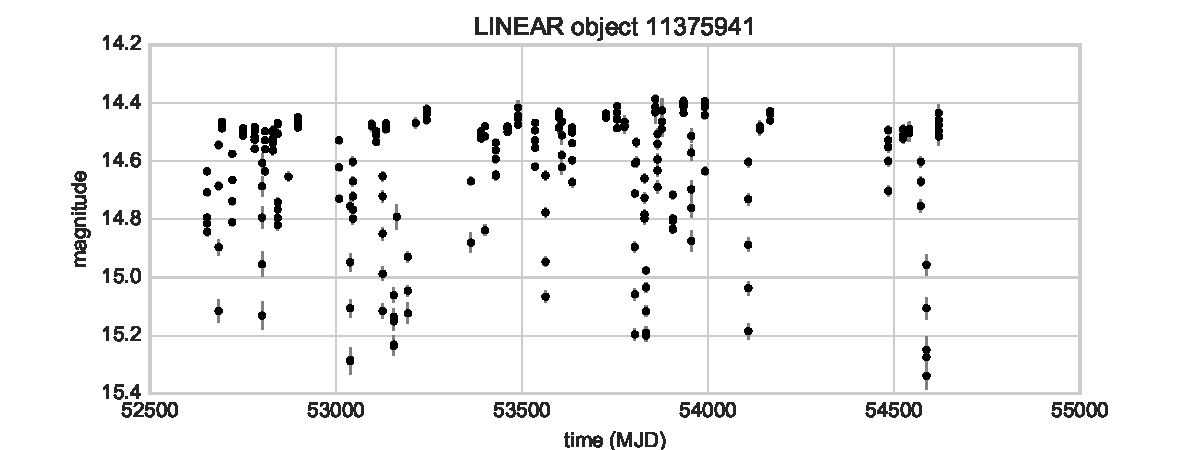
\includegraphics[width=\textwidth]{fig01_LINEAR_data}
\caption{Observed light curve from LINEAR object ID 11375941
    \figlabel{LINEAR_data}.
}
\end{figure}


\begin{figure}[ht]
\centering
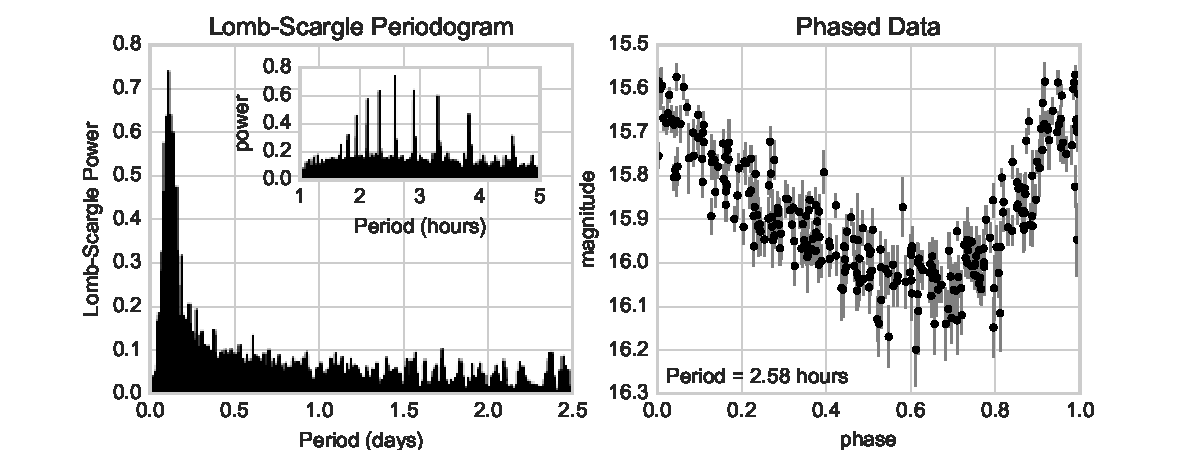
\includegraphics[width=\textwidth]{fig02_LINEAR_PSD}
\caption{{\it Left panel:} the Lomb-Scargle periodogram computed from the data
    in \fig{LINEAR_data}, with an inset detailing the interesting region.
    {\it Right panel:} the input data in \fig{LINEAR_data}, folded over the
    2.58-hour period to show the coherent periodic variability.
    \figlabel{LINEAR_power}
}
\end{figure}


\section{Background: Periods in Continuous Signals}

for a continuously defined signal $g(t)$, the Fourier transform is $\hat{g}(\nu)$,

\begin{equation}
    \mathcal{F}\left\{g\right\}(f) = \int_{-\infty}^\infty g(t) e^{-2\pi i f t} dt
\end{equation}

[Perhaps put this info in an appendix?]

Continuous signal $g(t)$:

\begin{equation}
  \mathcal{F}\left\{g\right\}(f) = \int_{-\infty}^\infty g(t) e^{-2\pi i f t} dt
\end{equation}

The inverse of this operation is

\begin{equation}
  \mathcal{F}^{-1}\left\{g\right\}(f) = \int_{-\infty}^\infty g(t) e^{+2\pi i f t} dt
\end{equation}

We can denote this

\begin{equation}
  \hat{g} = \mathcal{F}\left\{g\right\}
\end{equation}

\subsection{Important Properties of the CFT}

\subsubsection{Linearity}
The Fourier Transform is a linear operation, meaning that for two functions $f(t)$ and $g(t)$ and a scalar value $A$,

\begin{eqnarray}
  \mathcal{F}\{g + h\} &=& \mathcal{F}\{g\} + \mathcal{F}\{h\}\\
  \mathcal{F}\{A g\} &=& A\mathcal{F}\{g\}
\end{eqnarray}

These properties follow straightforwardly from the linearity of the Fourier transform definition.

\subsubsection{The Convolution Theorem}

The Fourier transform is central to an identity known as {\it the convolution theorem}.
The convolution of two functions $g(t)$ and $h(t)$ is itself a function of $t$, denoted $\{g \ast h\}(t)$, and is defined as

\begin{equation}
  \{g \ast h\}(t) \equiv \int_{-\infty}^\infty g(t - \tau) h(\tau) d\tau
\end{equation}

The convolution theorem states that the Fourier transform of a convolution is equal to the product of Fourier transforms; that is,

\begin{equation}
  \mathcal{F}\{g \ast h\} = \mathcal{F}\{g\}\mathcal{F}\{h\}
\end{equation}

This property can also be shown (relatively) straightforwardly from the convolution and Fourier transform definitions.

\subsubsection{$\mathcal{F}$ of a Gaussian is a Gaussian}
One of the special functions under a Fourier transform is the Gaussian distribution:

\begin{equation}
    g(t; \mu, \sigma) = \frac{1}{\sqrt{2\pi\sigma^2}} \exp\left[\frac{- (x - \mu)^2}{2\sigma^2}\right]
\end{equation}, which is proportional to


\subsubsection{$\mathcal{F}$ of a Periodic Function is a Delta Function}

A particularly special function in the complex exponential, $e^{2\pi i\nu_0 t} \equiv \cos(2\pi \nu_0 t) + i\sin(2\pi\nu_0 t)$, which has the Fourier transform $\mathcal{F}\{e^{2\pi i\nu_0 t}\} = \delta(\nu - \nu_0)$, which follows directly from the definition of the Dirac delta function:

\begin{equation}
  \delta(\nu) \equiv \int_{-\infty}^\infty e^{-2\pi i\nu t}dt
\end{equation}

Similarly, if we have a signal composed of a sum of complex exponentials, the linearity of the Fourier transform assures that the transform is simply a sum of delta functions:
\begin{equation}
  \mathcal{F}\left\{ \sum_{n=1}^N e^{-2\pi i \nu_n t} \right\} = \sum_{n=1}^N \delta(\nu - \nu_n)
\end{equation}
This result shows the sense in which a Fourier transform is an ideal measure of periodicity: the Fourier transform pulls-out and identifies the individual periodic components of any input.

\subsection{Fourier Power}

Using the above definitions, it is straightforward to show that a time-offset in a function leads to a multiplicative phase in the Fourier transform; that is, if
\begin{equation}
  g_\tau(t) \equiv g(t - \tau)
\end{equation}
then
\begin{equation}
  \mathcal{F}\{g_\tau\} = e^{-2\pi i \nu \tau}\mathcal{F}\{g\}
\end{equation}
Because the phase merely represents the chosen coordinate system, we'd like to remove it for spectral analysis.
One way to do this is to compute the power spectral density, which is proportional to \todo{const of proportionality?} the squared modulus of the Fourier Transform:
\begin{equation}
  P\{g\} \propto \left| \mathcal{F}\{g\} \right|^2.
\end{equation}
Because the modulus of a phase is equal to unity, the resulting measure is unchanged under time-translations in $g(t)$, and $P\{g\} = P\{g_\tau\}$ for any time-shift $\tau$.

\begin{itemize}
\item Some examples of functions, their transforms, and their power.
\end{itemize}

\subsection{Effect of Window Functions}

\begin{itemize}
\item convolution function and windowing
\end{itemize}

\section{From Idealistic to Realistic}

All of the above theory is beautiful and elegant, but when the theory meets the real world things get a bit more messy.
In particular, we rarely (if ever) are able to measure continuous functions like $g(t)$, but instead measure discrete realizations of the underlying function at a finite number of particular times $t_n$.
These discrete observations are effectively a window function over our data, and as we saw above, the presence of such a window function will propagate through our computation of the Fourier power!
The quantitative result of this windowning depends on the exact nature of the observation pattern; we will first consider the somewhat simpler case of evenly-spaced discrete data.

\subsection{Evenly-Spaced Discrete Data: the Schuster Periodogram}

Let's first consider the case of a large series of evenly-spaced observations.
Discrete samples can


\begin{itemize}
\item Evenly-spaced delta functions $\to$ evenly-spaced delta in frequency, separated by nyquist
\end{itemize}

\subsection{Unevenly-Spaced Discrete Data: the Lomb-Scargle Periodogram}


\begin{itemize}
\item Unevenly-spaced delta functions: no cancelations, and so window is generally {\it infinitely} wide.
\item Least-squares equivalence of Lomb-Scargle
\end{itemize}

\section{What Frequency Grid to Use?}

\begin{itemize}
\item Follow discussion from gatspy documentation
\end{itemize}

\section{Reporting errors in Frequency: Uncertainty vs. Precision}

\begin{itemize}
\item Talk about peak width and False Alarm Probability; recommend bootstrap (show example of when analytic FAP fails?)
\end{itemize}

\section{Algorithmic Considerations}

\begin{itemize}
\item Talk about Press \& Rybicki method; show some benchmarks.
\end{itemize}

\section{Generalizations \& Challenges}

\begin{itemize}
\item Multiterm makes the true period fit better, but also bumps the background noise.
\end{itemize}

\citet{VanderPlas2015}

\bibliographystyle{apj}
\bibliography{paper}

\end{document}
